% Elsevier elsarticle manuscript skeleton; content is added only after author approval.
% Source template: Desktop/论文修改/写作/elsarticle/elsarticle-template-num.tex
\documentclass[final,5p,times,twocolumn]{elsarticle}

\usepackage{amsmath,amssymb}
\usepackage{graphicx}
\usepackage{booktabs}
\usepackage{multirow}
\usepackage{algorithm}
\usepackage{algpseudocode}
\usepackage{float}
\usepackage{placeins}
\usepackage{needspace}
\usepackage{afterpage}
\usepackage{dblfloatfix}
\usepackage{multicol}
\usepackage{hyperref}
\hypersetup{hidelinks}
\usepackage{CJKutf8}
\usepackage{xcolor}
\newcommand{\purplerevision}[1]{#1}
\newcommand{\methodrevision}[1]{#1}
\newcommand{\nextrevision}[1]{#1}
\newcommand{\greenrevision}[1]{#1}
\newcommand{\redrevision}[1]{\textcolor{red}{#1}}
\newcommand{\fixedtablecaption}[1]{%
  \refstepcounter{table}%
  \par\smallskip\small Table~\thetable: #1\par\smallskip%
}
\newcommand{\fixedfigurecaption}[1]{%
  \refstepcounter{figure}%
  \par\smallskip\small Figure~\thefigure: #1\par\smallskip%
}
\newcommand{\methodframeworkfigure}{figures/method_overview_main4_picture3_20261003.png}
\newcommand{\methodframeworkwidth}{0.88\textwidth}

% Keep double-column floats close to their discussion and avoid sparse float pages.
\renewcommand{\topfraction}{0.95}
\renewcommand{\bottomfraction}{0.90}
\renewcommand{\textfraction}{0.05}
\renewcommand{\floatpagefraction}{0.80}
\renewcommand{\dbltopfraction}{0.95}
\renewcommand{\dblfloatpagefraction}{0.80}
\setlength{\textfloatsep}{10pt plus 2pt minus 2pt}
\setlength{\intextsep}{6pt plus 1pt minus 1pt}
\setlength{\dbltextfloatsep}{10pt plus 2pt minus 2pt}
\setcounter{topnumber}{1}
\setcounter{bottomnumber}{2}
\setcounter{totalnumber}{5}
\setcounter{dbltopnumber}{1}
\makeatletter
\setlength{\@fptop}{0pt}
\setlength{\@fpsep}{12pt}
\setlength{\@fpbot}{0pt plus 1fil}
\setlength{\@dblfptop}{0pt}
\setlength{\@dblfpsep}{12pt}
\setlength{\@dblfpbot}{0pt plus 1fil}
\makeatother

\journal{Knowledge-Based Systems}

\begin{document}
\raggedbottom
\begin{frontmatter}

\title{Sample-Adaptive Relational Knowledge Integration for Zero-Shot Audio Classification}

\author[inst1]{Kexin Zhang\fnref{equalcontrib}}
\ead{25461355022@stu.wzu.edu.cn}

\author[inst2]{Zhizhong Ma\fnref{equalcontrib}}
\ead{mazhizhong@wzut.edu.cn}

\author[inst2]{Yitian Lin}
\ead{yitian.lin@wzut.edu.cn}

\author[inst2]{Bingchen Lin\fnref{orcidlin}}
\ead{Bingchen.Lin@wzut.edu.cn}

\author[inst3]{Haihan Yang}
\ead{269964500@stu.cwnu.edu.cn}

\author[inst2]{Zhengqiu Weng\corref{corresponding}}
\ead{derisweng@wzut.edu.cn}

\author[inst1,inst4]{Hui Huang\corref{corresponding}}
\ead{huanghui@wzu.edu.cn}

\fntext[equalcontrib]{Kexin Zhang and Zhizhong Ma contributed equally to this work.}
\fntext[orcidlin]{ORCID: \href{https://orcid.org/0000-0002-7046-7189}{0000-0002-7046-7189}.}
\cortext[corresponding]{Corresponding authors: Zhengqiu Weng and Hui Huang.}

\affiliation[inst1]{organization={College of Computer Science and Artificial Intelligence, Wenzhou University},
  city={Wenzhou}, postcode={325035}, country={China}}
\affiliation[inst2]{organization={School of Data Science and Artificial Intelligence, Wenzhou University of Technology},
  city={Wenzhou}, postcode={325035}, country={China}}
\affiliation[inst3]{organization={School of Electronic Information Engineering, China West Normal University},
  city={Nanchong}, postcode={637009}, country={China}}
\affiliation[inst4]{organization={Wenzhou Turing Institute for Advanced Study in Artificial Intelligence},
  city={Wenzhou}, postcode={325035}, country={China}}

\begin{abstract}
Zero-shot audio classification reduces the need for labeled audio in a target task by matching audio with natural-language class descriptions. \redrevision{Knowledge graphs can supply semantic information absent from short class names. However, knowledge associated with a class may have limited value for distinguishing that class in a given audio sample.} \redrevision{Prompts formed by concatenating class names with retrieved tail entities leave the connecting relations implicit, expressing only part of the retrieved graph information.} We propose Sample-Adaptive Knowledge Integration (SAKI), which uses structured knowledge for zero-shot audio classification without updating the parameters of Contrastive Language--Audio Pretraining (CLAP)~\cite{elizalde2023clap}. Audio-Aligned Knowledge Verbalization (AAKV) converts graph triples into \greenrevision{descriptions of sounds} that preserve entity and relation semantics. \redrevision{SAKI then selects relations using class predictions computed separately for each relation from its evidence and the original CLAP scores.} Hierarchical Fusion aggregates the selected evidence within each class and combines it with the original CLAP score to rerank candidate classes. On five public audio datasets, SAKI improves Hit@1 by 2.08--12.73 percentage points and mean reciprocal rank (MRR) by 1.02--6.68 percentage points over our controlled reimplementation of iKnow-audio. \redrevision{These results support adapting graph evidence to individual audio samples through relation selection, constrained verbalization, and score fusion for zero-shot audio classification.}
\end{abstract}

\begin{keyword}
Zero-shot audio classification \sep CLAP \sep Audio-centric knowledge graph \sep Sample-level relation selection \sep Knowledge verbalization \sep Evidence fusion
\end{keyword}

\end{frontmatter}

\section{Introduction}\label{sec:introduction}

Zero-shot audio classification uses class semantics to recognize sound classes without training examples from the target task, reducing the need for annotated audio. Contrastive Language--Audio Pretraining (CLAP) learns a shared representation space through audio--text contrastive learning, allowing natural-language descriptions to define classes for sound classification~\cite{elizalde2023clap}. However, short class names provide limited semantic information. Sound sources, contexts, and relations to other events are often not fully expressed in the text input.

Prior studies have enriched class semantics through textual prompting and structured knowledge. ReCLAP rewrites training captions and generates custom class prompts to add acoustic and contextual information~\cite{ghosh2024reclap}. \redrevision{PAT uses audio from the downstream task to assign weights to prompts and combine them. It also aligns audio and text representations~\cite{seth2025pat}.} These approaches improve the use of class semantics through richer text and better representation alignment. Knowledge graphs explicitly represent associations between sound events. iKnow-audio constructs an Audio-centric Knowledge Graph (AKG) and retrieves tail entities associated with candidate classes through a curated set of relations. It concatenates the tail entities with class names to form \greenrevision{enriched prompts} and adjusts CLAP's class rankings~\cite{olvera-etal-2025-iknow}. This study shows that graph knowledge associated with classes can support audio classification. \redrevision{Using this knowledge for a given audio sample also requires assessing its discriminative value for that sample.}

Using graph knowledge for classification involves relation selection, textual expression, and score fusion. First, graph retrieval identifies knowledge associated with a candidate class, but this association alone does not establish its discriminative value for the current audio. The value of a relation may vary across audio samples, motivating relation selection based on predictions for the current input. Second, concatenating a class name and a tail entity retains both entities but leaves their connecting relation implicit. The resulting text therefore does not fully express the retrieved relational information. Text construction should preserve the relation's meaning while limiting additions unsupported by the triple. Finally, knowledge-augmented prompts provide additional evidence, but differ in how closely they match the current audio. \redrevision{Knowledge weakly related to the input audio may also alter candidate class rankings.} Knowledge augmentation therefore needs to retain the discriminative information in the original CLAP scores while using graph evidence to refine predictions.

We propose Sample-Adaptive Knowledge Integration (SAKI), which converts previously retrieved class-related knowledge into evidence for individual audio samples while keeping CLAP parameters unchanged. SAKI constructs knowledge text offline, then selects relations for the input audio during online inference. It combines knowledge scores with the original CLAP scores to rerank candidate classes.

The main contributions of this work are as follows:
\begin{itemize}
  \item We introduce sample-level relation selection using top-1 voting and top-two score gaps from the class predictions obtained for each relation. This selects relation sets for individual audio samples without additional training.
  \item We introduce Audio-Aligned Knowledge Verbalization (AAKV), which converts knowledge graph triples into descriptions of sounds while preserving relations between entities. These descriptions express relational information as text for audio--text matching.
  \item We develop Hierarchical Fusion to aggregate knowledge evidence within each class and combine the aggregated score with the original CLAP score through an explicit weight. \redrevision{This separates evidence aggregation from the weighting of knowledge evidence in the final class scores.}
\end{itemize}

We evaluate SAKI on five public audio datasets against our controlled reimplementation of iKnow-audio (iKnow\textsuperscript{\dag}). SAKI improves Hit@1 by 2.08--12.73 percentage points and mean reciprocal rank (MRR) by 1.02--6.68 percentage points. In the component ablation, SAKI achieves the highest unweighted mean Hit@1 and MRR across the five datasets. Comparisons of relation selection and knowledge verbalization further support the respective designs under the evaluated settings.

The remainder of this paper is organized as follows. Section~2 reviews related work, and Section~3 presents the SAKI framework and its core components. Section~4 reports the experimental setup, results, analyses, and limitations. Section~5 concludes the paper.

% !TeX root = ../main-4.tex
\section{Related work}\label{sec:related-work}

\greenrevision{We review audio--language models, sound semantic descriptions and textual prompting, and structured knowledge for audio classification. These research directions address cross-modal matching, the information supplied by class descriptions, and the use of relations in classification, respectively.}

\subsection{Zero-shot audio classification with audio--language models}

\greenrevision{Zero-shot audio classification relates audio representations to class semantics to recognize classes without training audio from the target classes. Xie et al. learn an acoustic--semantic projection through a bilinear compatibility framework, using semantic representations from pretrained language models~\cite{xie2021zero}. Cross-modal pretraining provides a complementary route to natural-language supervision. CLIP learns transferable visual representations from image--text pairs~\cite{radford2021learning}. AudioCLIP incorporates an audio encoder into CLIP, whereas Wav2CLIP learns audio representations by distilling CLIP's visual representations~\cite{guzhov2021audioclip,wu2022wav2clip}. Both support matching audio with images and text in a shared embedding space.}

\greenrevision{Direct audio--text pretraining further develops this approach. CLAP uses two encoders and contrastive learning to map audio and text descriptions into a joint embedding space~\cite{elizalde2023clap}. LAION-CLAP expands the training data and introduces feature fusion and keyword-to-caption augmentation~\cite{wu2023clap}. M2D-CLAP combines masked audio modeling with audio--text alignment, while SLAP supports variable audio durations through joint contrastive, self-supervised, and captioning objectives~\cite{niizumi2024m2dclap,mei2026slap}. These studies strengthen the representations used for cross-modal matching. The semantic content of class descriptions also influences prediction, motivating the description and prompting methods reviewed below.}

\subsection{Sound semantic description and textual prompting}

\greenrevision{Sound semantic descriptions supply information beyond class names. Binary Attribute Embeddings represents classes through attributes such as pitch, duration, and source material~\cite{lin2022binary}. Sound Attribute Vector learns discriminative global features alongside spectrotemporal local features that predict attribute information~\cite{lin2023soundattribute}. Xu et al. use the knowledge of large language models to generate detailed auditory attribute descriptions for each class~\cite{xu2024soundattribute}. ReCLAP extends natural-language descriptions by training CLAP on rewritten audio captions and augmenting class prompts with sound descriptions in diverse scenes~\cite{ghosh2024reclap}. Attribute representations and textual descriptions thus provide different ways to supplement the semantics of short labels.}

\greenrevision{Prompting methods also consider task information and cross-modal alignment. TSPE constructs task-specific prompt ensembles using labels, sound attributes, and sound sources, then averages the prompt embeddings for each class~\cite{anand2025tspe}. For each prompt, PAT sums the maximum class prediction logit across audio samples from the downstream task. It uses these sums to weight and ensemble text representations. Its cross-modal alignment module uses attention between frame-level audio representations and text~\cite{seth2025pat}. In the related domain of sound design, AudioCards structures acoustic attributes and sonic descriptors as metadata for text--audio retrieval, descriptive captioning, and metadata generation~\cite{sridhar2026audiocards}. PAT's prompt weighting uses information across a task, while AudioCards addresses sound-design tasks rather than zero-shot class reranking.}

\greenrevision{These methods enrich attributes, descriptions, or prompt representations. Graph triples introduce a further requirement: the text needs to express the relation connecting the head and tail entities. Concatenating their names leaves this relation unstated, whereas unconstrained expansion may add content absent from the triple. AAKV therefore verbalizes the supplied entities and directed relation as a description of sound under explicit content constraints.}

% Queue the method overview early so it appears at the top of page 3.
\providecommand{\methodframeworkfigure}{figures/saki_framework.png}
\providecommand{\methodframeworkwidth}{0.96\textwidth}
\begin{figure*}[!t]
  \centering
  \includegraphics[width=\methodframeworkwidth]{\methodframeworkfigure}
  \caption{Overview of SAKI. Offline, class-to-entity mapping, RotatE tail retrieval, and AAKV produce cached graph evidence and CLAP text embeddings. Online, (a) CLAP identifies the top-$K$ classes; (b) \redrevision{class rankings computed separately for each relation provide top-1 predictions and top-two score gaps for sample-level relation selection}; and (c) the selected evidence is deduplicated and aggregated by class before fusion with the original CLAP score. Classes outside the initial top-$K$ or without usable evidence retain their original CLAP scores.}
  \label{fig:framework}
\end{figure*}

\subsection{Structured knowledge for audio classification}

\greenrevision{Structured knowledge represents class hierarchies and relations among audio events. AudioSet organizes sound classes through a hierarchical ontology~\cite{gemmeke2017audioset}. Jimenez et al. design neural architectures that preserve ontology structure~\cite{jimenez2018ontology}. Sun et al. combine feed-forward ontology layers with graph convolution to model label dependencies across and within ontology levels~\cite{sun2020ontology}. Aironi et al. compare node embeddings in a classification framework whose label graph is derived from label co-occurrence in training data~\cite{aironi2022graph}. Hou et al. construct event relational graphs for acoustic scene classification, representing events as nodes and pairwise relationship cues as multidimensional edge features~\cite{hou2023audio}. These approaches incorporate class or event structure into model learning; retrieving external graph evidence during audio--language inference involves a different process for using knowledge.}

\greenrevision{Knowledge graph embeddings enable relational retrieval through triple scores. RotatE represents each relation as a rotation from the head entity to the tail entity in complex space for link prediction~\cite{sun2019rotate}. iKnow-audio applies this retrieval process to CLAP's initial class predictions using a curated subset of informative relations. It concatenates class labels with retrieved tail entities to form enriched prompts, then jointly aggregates the original and enriched prompt scores through log-sum-exp~\cite{olvera-etal-2025-iknow}. Its graph scores assess entity--relation compatibility, while its initial candidates depend on the audio. SAKI further evaluates relations using predictions for the current audio and separates aggregation of knowledge evidence from fusion with the original CLAP score.}

\greenrevision{Input-dependent knowledge selection has also been studied in image classification. SINet selects graph knowledge through an attention-based module and uses a knowledge selection loss to measure consistency between knowledge and image features~\cite{tang2023sinet}. It offers a related example of selecting knowledge for an input, but learns the selection module within an image classification framework. SAKI selects relations using top-1 voting and top-two score gaps without training a selector on the target datasets.}

\greenrevision{Together, these research directions provide cross-modal representations, richer class semantics, and explicit relational knowledge. SAKI builds on this foundation to organize graph knowledge for individual audio samples at inference. The Sample-level Relation Selector determines which relations contribute evidence, AAKV expresses their triples under content constraints, and Hierarchical Fusion combines that evidence with the original CLAP prediction.}

% !TeX root = ../main-4.tex
\section{Method}\label{sec:method}

SAKI performs zero-shot audio classification without training on the target datasets. \redrevision{Figure~\ref{fig:framework} shows the offline knowledge preparation and online inference stages.} Offline, we map classes to graph entities, \redrevision{retrieve tail entities with RotatE}, verbalize the triples with Audio-Aligned Knowledge Verbalization (AAKV), and cache the graph evidence and CLAP text embeddings. Online, CLAP scores all classes and identifies the top-$K$ candidates for knowledge enhancement. \redrevision{For each relation, we combine scores from its cached evidence with the original CLAP scores. The resulting class ranking yields a top-1 prediction and a top-two score gap. These calculations use the same frozen CLAP model and require no separate training.} The Sample-level Relation Selector uses top-1 voting and the score gaps to rank relations for the current audio. Hierarchical Fusion then deduplicates and aggregates the selected graph evidence by class before combining it with the original CLAP score.

\subsection{Problem formulation}\label{sec:problem-formulation}

Given audio input $x^a$ and $N$ candidate classes $\mathcal C=\{c_1,c_2,\ldots,c_N\}$, the method assigns a final class score to every candidate and predicts
\begin{equation}
\hat y=\arg\max_{c_i\in\mathcal C}s_{\mathrm{final}}(c_i\mid x^a),
\label{eq:prediction}
\end{equation}
where $\hat y$ is the predicted class and $s_{\mathrm{final}}(c_i\mid x^a)$ \redrevision{is the final score assigned to class $c_i$.} We use the pretrained CLAP audio encoder $f_a(\cdot)$ and text encoder $f_t(\cdot)$. The Audio-centric Knowledge Graph is $\mathcal G=(\mathcal E,\mathcal R,\mathcal T)$, where $\mathcal E$, $\mathcal R$, and $\mathcal T$ denote the entity, relation, and triple sets. The principal notation is summarized below.

\par\smallskip\noindent\begin{minipage}{\columnwidth}
\centering
\textbf{Principal notation}\par\smallskip
\footnotesize
\setlength{\tabcolsep}{4pt}
\begin{tabular}{@{}p{0.37\columnwidth}p{0.55\columnwidth}@{}}
\toprule
Symbol & Meaning \\
\midrule
$x^a,\mathcal C,c_i$ & Input audio, candidate class set, and a candidate class \\
$\mathcal G,\mathcal E,\mathcal R$ & Knowledge graph, entity set, and relation set \\
$K,M,N_r$ & \redrevision{Numbers of shortlisted classes, maximum tail entities per class--relation pair, and selected relations} \\
$s_{\mathrm{base}},s_r,s_{\mathrm{final}}$ & Original CLAP score, relation-specific class score, and final class score \\
$\mathcal E_{i,r},\mathcal U_{i,r}$ & Retained tails and evidence scores for a class--relation pair \\
$\mathcal U_i^*$ & Evidence scores after merging selected relations and removing duplicate tails \\
$A_{\lambda},\lambda$ & Evidence aggregation operator and its fixed scale \\
$\mathcal F,\alpha$ & Two-step scoring rule and weight on the original CLAP score \\
\bottomrule
\end{tabular}
\end{minipage}\par\smallskip

\subsection{CLAP initial retrieval and graph evidence construction}\label{sec:initial-retrieval}

For input audio $x^a$ and class text $c_i$, we $L_2$-normalize the CLAP audio and text representations and denote them by $\mathbf e^a$ and $\mathbf e_i^t$. Their audio--text similarity gives the original CLAP score~\cite{elizalde2023clap}:
\begin{equation}
s_{\mathrm{base}}(c_i\mid x^a)=(\mathbf e^a)^\top\mathbf e_i^t.
\label{eq:base-score}
\end{equation}
We rank all classes by $s_{\mathrm{base}}$ and select the $K$ classes eligible for graph augmentation:
\begin{equation}
\mathcal C_K(x^a)=\operatorname{TopK}_{c_i\in\mathcal C}s_{\mathrm{base}}(c_i\mid x^a).
\label{eq:topk}
\end{equation}
Classes outside $\mathcal C_K$ retain their original CLAP scores and remain in the final ranking.

A verified class-to-entity mapping assigns class $c_i$ to a graph head entity $h_i\in\mathcal E$. Classes without a mapping receive no graph evidence. Following the knowledge retrieval setup of iKnow-audio, we score candidate triples with a pretrained RotatE knowledge graph embedding (KGE) model~\cite{olvera-etal-2025-iknow,sun2019rotate}. For $h_i\in\mathcal E$, $r\in\mathcal R$, and $t\in\mathcal E$, the score $\phi_{\mathrm{KG}}(h_i,r,t)$ \redrevision{measures the plausibility of triple $(h_i,r,t)$ under the embedding model.} RotatE uses $\phi_{\mathrm{KG}}(h_i,r,t)=-\|\mathbf h_i\circ\mathbf r-\mathbf t\|_2$, where bold symbols denote embeddings and $\circ$ denotes elementwise multiplication. \greenrevision{Entity and relation embeddings are complex-valued, with unit-modulus relation components.} A higher score indicates a more plausible triple under the embedding model. We retain the $M$ highest-scoring tail entities:
\begin{equation}
\widetilde{\mathcal E}_{i,r}^{M}=\operatorname{TopM}_{t\in\mathcal E}\phi_{\mathrm{KG}}(h_i,r,t).
\label{eq:tail-retrieval}
\end{equation}
\greenrevision{We remove tails whose normalized names match any class in $\mathcal C$ and deduplicate the remaining tails using lowercase strings with leading and trailing whitespace removed. The retained set is $\mathcal E_{i,r}$, with $|\mathcal E_{i,r}|\leq M$; removed tails are not replaced. For an unmapped class or an empty filtered result, $\mathcal E_{i,r}=\varnothing$.} Retrieval is performed offline for every mapped class and each of the 47 candidate relations. Online inference reads the cached evidence only for classes in $\mathcal C_K$.

\subsection{Audio-Aligned Knowledge Verbalization}\label{sec:aakv-method}

\greenrevision{AAKV verbalizes each retrieved graph triple $(h_i,r,t)$ as $q_{irt}$, using the corresponding class name $c_i$ as the supplied head text. The graph entity $h_i$ is used for retrieval; the class name $c_i$ is used in the generated description. }The term \emph{audio-aligned} describes \greenrevision{text about sounds intended for CLAP audio--text matching}; generation is not conditioned on the input audio. The instruction requires the sentence to begin with the words \textit{The sound of} followed by the supplied head text. It also requires the original entity wording, relation meaning and direction, and tail entity to be retained without adding information beyond the triple.

We generate the text offline with Qwen2.5-7B-Instruct using greedy decoding. \redrevision{Rule-based checks test the normalized prefix, coverage of head and tail content words, and terms denoting the relation. They also check output length, line and sentence formatting, and predefined prohibited expressions.} If the output fails, we attempt one constrained repair using \greenrevision{the reasons for failure}. A second failure triggers a deterministic template that inserts the supplied head, relation, and tail text. \ref{app:aakv-protocol} specifies the exact instruction, checks, and fallback. This procedure constrains the expression of graph evidence to the information in the input triple.

We encode each accepted text with the same CLAP text encoder and $L_2$-normalize its embedding:
\begin{equation}
\mathbf z_{irt}=\frac{f_t(q_{irt})}{\|f_t(q_{irt})\|_2},\qquad u_{irt}(x^a)=(\mathbf e^a)^\top\mathbf z_{irt}.
\label{eq:evidence-score}
\end{equation}
Here $\mathbf z_{irt}$ is the cached text embedding, and $u_{irt}(x^a)$ is its audio--text similarity for the current sample. All $\mathbf z_{irt}$ are computed before online inference.

\subsection{Sample-level relation selection}\label{sec:relation-selector-method}

\redrevision{For each relation $r$, we compute class scores using only the cached evidence associated with that relation and the original CLAP scores.} We first aggregate the evidence scores within one class. \greenrevision{For $\mathcal U=(u_1,\ldots,u_n)$, where $u_j$ is the audio--text similarity of evidence item $j$ ($j=1,\ldots,n$), we use the normalized scaled log-sum-exp operator~\cite{asadi2017softmax}:}
\begin{equation}
A_{\lambda}(\mathcal U)=\frac{1}{\lambda}\log\left(\frac{1}{n}\sum_{j=1}^{n}\exp(\lambda u_j)\right),\qquad n>0.
\label{eq:normlse}
\end{equation}
\greenrevision{The factor $1/n$ removes the additive count term of unnormalized log-sum-exp. The fixed scale $\lambda>0$ controls the emphasis on higher-scoring items: $A_{\lambda}$ lies between their arithmetic mean and maximum and approaches the maximum as $\lambda$ increases. This operator aggregates graph evidence only.}

\Needspace{5\baselineskip}
\greenrevision{For a shortlisted class with nonempty evidence, we combine its knowledge score with the original CLAP score as follows:}
\begin{equation}
\greenrevision{\begin{aligned}
\mathcal F(c_i,\mathcal U\mid x^a)
&=\alpha s_{\mathrm{base}}(c_i\mid x^a)\\
&\quad +(1-\alpha)A_{\lambda}(\mathcal U).
\end{aligned}}
\label{eq:unified-fusion}
\end{equation}
\greenrevision{Here $\alpha\in[0,1]$ weights the original CLAP score. For $c_i\notin\mathcal C_K$ or $\mathcal U=\varnothing$, we define $\mathcal F(c_i,\mathcal U\mid x^a)=s_{\mathrm{base}}(c_i\mid x^a)$.}

\redrevision{For class $c_i$ and relation $r$, we collect the evidence scores} $\mathcal U_{i,r}(x^a)=[u_{irt}(x^a)\mid t\in\mathcal E_{i,r}]$. Applying Eq.~\eqref{eq:unified-fusion} to this single-relation sequence yields its relation-specific class score:
\[
s_r(c_i\mid x^a)=\mathcal F(c_i,\mathcal U_{i,r}(x^a)\mid x^a).
\]
\redrevision{For each relation, we rank all candidate classes by $s_r$. The resulting top-1 prediction $\hat y_r$ and top-two score gap $\Delta_r$ are}
\begin{equation}
\hat y_r=\arg\max_{c_i\in\mathcal C}s_r(c_i\mid x^a),\qquad \Delta_r=s_r^{(1)}-s_r^{(2)},
\label{eq:expert-margin}
\end{equation}
where $s_r^{(1)}$ and $s_r^{(2)}$ \redrevision{are the highest and second-highest values of $s_r$.} \greenrevision{Ties in the top-1 prediction are resolved by the lower index in the fixed candidate class list.} If relation $r$ provides no usable evidence for any class in $\mathcal C_K$, \redrevision{$s_r$ equals the original CLAP score for every class, and the resulting top-1 prediction still participates in voting.}

For the current audio, we count the top-1 votes received by each class:
\begin{equation}
V(c)=\sum_{r\in\mathcal R}\mathbb I(\hat y_r=c),
\label{eq:voting}
\end{equation}
where $\mathbb I(\cdot)$ equals one when the condition holds and zero otherwise. The consensus class has the most votes. \redrevision{For tied classes, we first choose the larger sum of score gaps from relations whose top-1 predictions support that class. Any remaining tie is resolved by the lower index in the fixed candidate class list:}
\begin{equation}
c^{\mathrm{con}}=\arg\max_{c\in\mathcal C}^{\mathrm{lex}}\left(V(c),\sum_{r:\hat y_r=c}\Delta_r,-\operatorname{idx}(c)\right).
\label{eq:consensus}
\end{equation}
Here $\arg\max^{\mathrm{lex}}$ compares tuple components from left to right. We then rank relations using
\begin{equation}
\begin{array}{@{}l@{\;=\;}l@{}}
\pi_r & \left(\mathbb I(\hat y_r=c^{\mathrm{con}}),\,\Delta_r,\,-\operatorname{idx}(r)\right),\\[2pt]
\mathcal R^*(x^a) & \operatorname{Top}_{N_r}^{\mathrm{lex}}(\mathcal R;\pi).
\end{array}
\label{eq:relation-selection}
\end{equation}
Relations supporting the consensus class come first. Within the supporting and nonsupporting groups, relations are ordered by decreasing $\Delta_r$. Remaining ties follow the fixed lexicographic order of relation names, encoded by $\operatorname{idx}(r)$. The first $N_r$ relations form the ordered selection $\mathcal R^*(x^a)$; nonsupporting relations fill any remaining positions. \greenrevision{The selected relations are shared by all classes in $\mathcal C_K$.} We select $N_r$ from $\{1,3,5,10\}$ on the development set, fix it at $5$, and use the same value on every test dataset.

\subsection{Hierarchical Fusion}\label{sec:fusion-method}

After relation selection, we process each class in $\mathcal C_K$ separately. In the priority order of Eq.~\eqref{eq:relation-selection}, we collect evidence from the selected relations. Duplicate tails across these relations are identified using the normalized tail-entity string. When a tail appears under several relations, we retain the AAKV text associated with the highest-priority relation. Let $\mathcal P_i(x^a)=[(r,t,q_{irt})]$ be the retained evidence sequence. Its audio--text similarity scores are
\begin{equation}
\mathcal U_i^*(x^a)=\left[u_{irt}(x^a)\mid(r,t,q_{irt})\in\mathcal P_i(x^a)\right].
\label{eq:selected-evidence}
\end{equation}
Each selected relation supplies at most $M$ evidence items per class. Thus, there are at most $MN_r$ items before deduplication, and $\mathcal U_i^*$ contains all retained items after deduplication.

\greenrevision{At final scoring, Eq.~\eqref{eq:unified-fusion} combines the merged evidence sequence with the original CLAP score, rather than with a relation-specific score:}
\[
s_{\mathrm{final}}(c_i\mid x^a)=\mathcal F(c_i,\mathcal U_i^*(x^a)\mid x^a).
\]
Classes outside $\mathcal C_K$, without an entity mapping, or without usable evidence retain $s_{\mathrm{base}}$. We then rank every class by $s_{\mathrm{final}}$ and predict with Eq.~\eqref{eq:prediction}. Algorithm~\ref{alg:relation-selection} summarizes online inference. Its first loop scores each relation using cached evidence; after relation selection, the second loop merges the selected evidence and computes final class scores. RotatE retrieval and AAKV are offline and are not repeated in this algorithm.

\begin{algorithm}[H]
\caption{Online inference with sample-level relation selection and Hierarchical Fusion}
\label{alg:relation-selection}
\fontsize{7}{10}\selectfont
\begin{algorithmic}[1]
\Require Audio $x^a$; classes $\mathcal C$; relations $\mathcal R$; cached evidence $\{\mathcal E_{i,r},\mathbf z_{irt}\}$; $K,N_r,\alpha,\lambda$
\Ensure Final class scores, class ranking, and prediction $\hat y$
\State Encode $x^a$ as $\mathbf e^a$, and compute $s_{\mathrm{base}}(c_i\mid x^a)$ by Eq.~\eqref{eq:base-score}
\State Select $\mathcal C_K$ by Eq.~\eqref{eq:topk}
\For{$r\in\mathcal R$}
  \For{$c_i\in\mathcal C_K$}
    \State Construct $\mathcal U_{i,r}(x^a)\gets[u_{irt}(x^a)\mid t\in\mathcal E_{i,r}]$ by Eq.~\eqref{eq:evidence-score}
    \State Compute $s_r(c_i\mid x^a)\gets\mathcal F(c_i,\mathcal U_{i,r}(x^a)\mid x^a)$
  \EndFor
  \State Keep $s_r(c_i\mid x^a)\gets s_{\mathrm{base}}(c_i\mid x^a)$ for $c_i\notin\mathcal C_K$
  \State Obtain $(\hat y_r,\Delta_r)$ by Eq.~\eqref{eq:expert-margin}
\EndFor
\State Compute $V(c)$ and determine $c^{\mathrm{con}}$ by Eqs.~\eqref{eq:voting}--\eqref{eq:consensus}
\State Rank $\mathcal R$ by $\pi_r$ and retain $\mathcal R^*(x^a)$ using Eq.~\eqref{eq:relation-selection}
\For{$c_i\in\mathcal C_K$}
  \State Merge selected evidence in \greenrevision{order of relation priority} and remove duplicate tails
  \State Construct $\mathcal U_i^*(x^a)$ by Eq.~\eqref{eq:selected-evidence}
  \State Compute $s_{\mathrm{final}}(c_i\mid x^a)$ by Eq.~\eqref{eq:unified-fusion}
\EndFor
\State Keep $s_{\mathrm{final}}(c_i\mid x^a)\gets s_{\mathrm{base}}(c_i\mid x^a)$ for $c_i\notin\mathcal C_K$
\State Rank $\mathcal C$ by $s_{\mathrm{final}}$ and set $\hat y\gets\arg\max_{c_i\in\mathcal C}s_{\mathrm{final}}(c_i\mid x^a)$
\State \textbf{return} final class scores, ranking, and $\hat y$
\end{algorithmic}
\end{algorithm}

All experiments use $K=5$, $M=3$, and $\lambda=100$. The \greenrevision{values $\alpha=0.3$ and $N_r=5$ chosen on the development set} remain fixed across test datasets. The candidate pool contains 47 relations. CLAP and RotatE parameters are unchanged throughout, with no gradient updates on the target audio data.

% !TeX root = ../main-4.tex
\providecommand{\nextrevision}[1]{#1}
\section{Experiments}\label{sec:experiments}


\subsection{Experimental setup}\label{sec:setup}

\subsubsection{Datasets}\label{sec:datasets}

We evaluate SAKI on five public audio classification datasets: \greenrevision{ESC-50~\cite{piczak2015esc}, UrbanSound8K~\cite{salamon2014urbansound}, TUT Acoustic Scenes 2017 (TUT2017)~\cite{mesaros2016tut,mesaros2017dcase}, FSD50K~\cite{fonseca2022fsd50k}, and AudioSet~\cite{gemmeke2017audioset}}. ESC-50 contains 2,000 five-second clips from 50 environmental sound classes. UrbanSound8K contains 8,732 clips of up to four seconds from 10 urban sound classes. \greenrevision{For TUT2017, we combine 4,680 development and 1,620 evaluation clips, yielding 6,300 ten-second clips from 15 acoustic scene classes.} For FSD50K, we use the 10,231 clips in the official evaluation split and all 200 candidate classes. For AudioSet, we use its 527-class evaluation label space and 17,233 publicly accessible audio files that can be decoded. ESC-50, UrbanSound8K, and TUT2017 are single-label datasets; FSD50K and AudioSet are multilabel datasets.

We use \greenrevision{DCASE17-T4~\cite{mesaros2017dcase}} as a development set. It contains 419 publicly accessible, decodable clips from 17 sound event classes. Development labels are used only to select the fusion weight and the number of relations. These parameters are then fixed for all five test datasets. Test labels are used only to compute evaluation metrics, with no role in training, knowledge retrieval, text generation, or relation selection.






\subsubsection{Comparison methods}\label{sec:comparison-methods}

\greenrevision{The comparison includes the following three methods:}

\begin{enumerate}
    \item \textbf{CLAP}: \redrevision{CLAP serves as the knowledge-free baseline. Its pretrained encoders compute similarities between the input audio and candidate class texts without external knowledge.}
    \item \textbf{iKnow\textsuperscript{\dag}}: \redrevision{Our controlled reimplementation of iKnow-audio serves as the knowledge-enhanced baseline.}
    \item \textbf{SAKI}: Our method comprises AAKV, the Sample-level Relation Selector, and Hierarchical Fusion, as described in Section~\ref{sec:method}.
\end{enumerate}

\bluerevision{The paper describes the inference procedure, but the complete curated relation subset $R_q$ and classification inference implementation are not publicly available~\cite{olvera-etal-2025-iknow}. We therefore evaluate a controlled reimplementation under our common protocol.} It is a controlled reimplementation rather than an exact replication of the original system. The protocol and dataset differences are \redrevision{documented in \ref{app:reproduction}.} All internal comparisons use identical test manifests and evaluation code.

\subsubsection{Implementation details}\label{sec:implementation-details}

We use MS-CLAP 2023 as the audio--text backbone and pretrained RotatE for knowledge graph tail prediction. CLAP and RotatE parameters remain unchanged throughout the experiments. Candidate class labels are lowercased, and underscores are replaced with spaces \redrevision{to standardize class label formatting.}

For consistent internal comparisons, we set $K=5$, $M=3$, and $\lambda=100$ in iKnow\textsuperscript{\dag} and all subsequent ablations. Here, $K$ is the number of classes shortlisted by CLAP, and \redrevision{$M$ is the maximum number of tail entities retained for each class--relation pair.} The controlled reimplementation uses normalized scaled log-sum-exp aggregation to reduce aggregation shifts caused by differences in evidence counts. This setting is retained across the experimental configurations.

We use the AKG constructed by iKnow-audio and its 47 relation types as the common candidate relation pool. For classes mapped to the graph, pretrained RotatE retrieves candidate tails for each class--relation pair offline. AAKV uses Qwen2.5-7B-Instruct with greedy decoding. The generated knowledge texts and their CLAP text embeddings are cached before audio inference.

During online inference, CLAP scores all candidate classes and retains the top $K$. SAKI then selects $N_r$ relations according to Section~\ref{sec:relation-selector-method} and combines their evidence with the original CLAP scores.

We select the fusion weight $\alpha$ and the number of relations $N_r$ by grid search on the DCASE17-T4 development set:
\begin{equation}
\alpha\in\{0.3,0.5,0.7\},\qquad
N_r\in\{1,3,5,10\}.
\end{equation}
Configurations are compared first by development Hit@1 and then, in a tie, by MRR. If both metrics are equal, we select the smaller number of relations. The resulting settings, $\alpha=0.3$ and $N_r=5$, are fixed for all five test datasets.

Audio is resampled to 44.1~kHz and processed into seven-second segments. \greenrevision{Shorter clips are repeated to reach seven seconds. For longer clips, MS-CLAP randomly chooses a starting point and extracts one continuous seven-second segment. A seed derived from the fixed value 42 and each audio path makes this choice reproducible; all methods use the same cached audio representation for each sample.} We run the experiments on a server with three NVIDIA GeForce RTX 4090 D GPUs. The software environment comprises Ubuntu 22.04, Python 3.10.19, PyTorch 2.4.0, CUDA 12.1, MS-CLAP 1.3.4, Transformers 4.57.6, and PyKEEN 1.11.1.



\subsubsection{Evaluation metrics}\label{sec:evaluation-metrics}

We report Hit@$k$ and mean reciprocal rank (MRR). Hit@$k$ is the proportion of samples with at least one ground-truth label among the top $k$ classes; we report Hit@1, Hit@3, and Hit@5. \redrevision{MRR averages the reciprocal rank of the highest-ranked ground-truth label in the complete class ranking.} For multilabel samples, all ground-truth labels are positive, and the highest-ranked positive label determines the reciprocal rank. All metrics are reported as percentages, with higher values indicating better performance.

\bluerevision{For each metric, the mean across the five datasets is the arithmetic mean of the five dataset scores, without weighting by sample count.}

To assess the uncertainty of performance differences, we compute 95\% confidence intervals using 10,000 paired bootstrap resamples of the sample-level predictions. For Hit@1, we also apply two-sided exact McNemar tests to paired correctness outcomes and use Holm adjustment for comparisons across the five datasets.

All reported performance differences are computed from unrounded metric values and rounded to two decimal places for presentation.



\twocolumn[{
\begin{minipage}{\textwidth}
\begin{table}[H]
\centering
\caption{Results (\%) for CLAP, iKnow\textsuperscript{\dag}, and SAKI on five zero-shot audio classification test datasets. Higher is better; bold indicates the highest value for each dataset and metric. \textsuperscript{\dag} denotes our controlled reimplementation of iKnow-audio. All three methods use identical test samples.}
\label{tab:main-results}
\setlength{\tabcolsep}{3.5pt}
\resizebox{\textwidth}{!}{%
\begin{tabular}{l*{15}{c}}
\toprule
\multirow{2}{*}{Metric}
& \multicolumn{3}{c}{ESC-50}
& \multicolumn{3}{c}{UrbanSound8K}
& \multicolumn{3}{c}{FSD50K}
& \multicolumn{3}{c}{AudioSet}
& \multicolumn{3}{c}{TUT2017} \\
\cmidrule(lr){2-4}\cmidrule(lr){5-7}\cmidrule(lr){8-10}\cmidrule(lr){11-13}\cmidrule(lr){14-16}
& CLAP & iKnow\textsuperscript{\dag} & SAKI
& CLAP & iKnow\textsuperscript{\dag} & SAKI
& CLAP & iKnow\textsuperscript{\dag} & SAKI
& CLAP & iKnow\textsuperscript{\dag} & SAKI
& CLAP & iKnow\textsuperscript{\dag} & SAKI \\
\midrule
Hit@1
& 91.10 & 91.75 & \textbf{94.25}
& 83.76 & 84.88 & \textbf{87.17}
& 57.35 & 59.84 & \methodrevision{\textbf{64.46}}
& 28.65 & 29.22 & \methodrevision{\textbf{31.29}}
& 40.65 & 44.14 & \textbf{56.87} \\
Hit@3
& 96.75 & \textbf{97.05} & 96.80
& 96.60 & 96.77 & \textbf{96.90}
& 79.65 & \textbf{80.73} & \methodrevision{80.52}
& 46.36 & \textbf{47.04} & \methodrevision{46.90}
& 76.59 & 79.89 & \textbf{80.54} \\
Hit@5
& \textbf{97.65} & \textbf{97.65} & \textbf{97.65}
& \textbf{98.65} & \textbf{98.65} & \textbf{98.65}
& 86.35 & \textbf{86.51} & \methodrevision{86.48}
& 54.80 & \textbf{54.87} & \methodrevision{54.80}
& 92.24 & \textbf{92.68} & 91.79 \\
MRR
& 94.11 & 94.57 & \textbf{95.75}
& 90.40 & 91.08 & \textbf{92.22}
& 70.17 & 71.80 & \methodrevision{\textbf{74.13}}
& 41.06 & 41.54 & \methodrevision{\textbf{42.56}}
& 60.79 & 64.04 & \textbf{70.73} \\
\bottomrule
\end{tabular}
}

\end{table}
\vspace{8pt}
\begin{table}[H]
\centering
\caption{Component ablations (\%, Hit@1/MRR). The plus sign denotes a component added to iKnow\textsuperscript{\dag}. \greenrevision{The mean across the five datasets is the unweighted arithmetic mean of their metrics.} Fusion and Selector abbreviate Hierarchical Fusion and Sample-level Relation Selector. Bold indicates the highest value in each column.}
\label{tab:factorial-ablation}
\setlength{\tabcolsep}{2.5pt}
\resizebox{\textwidth}{!}{%
\begin{tabular}{l*{12}{c}}
\toprule
\multirow{2}{*}{Method}
& \multicolumn{2}{c}{ESC-50}
& \multicolumn{2}{c}{UrbanSound8K}
& \multicolumn{2}{c}{FSD50K}
& \multicolumn{2}{c}{AudioSet}
& \multicolumn{2}{c}{TUT2017}
& \multicolumn{2}{c}{\greenrevision{Mean (5 datasets)}} \\
\cmidrule(lr){2-3}\cmidrule(lr){4-5}\cmidrule(lr){6-7}\cmidrule(lr){8-9}\cmidrule(lr){10-11}\cmidrule(lr){12-13}
& Hit@1 & MRR & Hit@1 & MRR & Hit@1 & MRR & Hit@1 & MRR & Hit@1 & MRR & Hit@1 & MRR \\
\midrule
iKnow\textsuperscript{\dag}
& 91.75 & 94.57 & 84.88 & 91.08 & 59.84 & 71.80 & 29.22 & 41.54 & 44.14 & 64.04 & 61.97 & 72.61 \\
+ AAKV
& 88.65 & 92.63 & 84.52 & 90.59 & 61.60 & 72.65 & 28.65 & 41.16 & 48.68 & 66.20 & 62.42 & 72.65 \\
+ Fusion
& 92.85 & 95.15 & 85.02 & 91.18 & 60.83 & 72.49 & 29.64 & 41.88 & 46.86 & 65.86 & 63.04 & 73.31 \\
+ Selector
& 93.85 & 95.63 & 85.83 & 91.44 & 60.29 & 71.88 & 29.87 & 41.77 & 46.56 & 65.39 & 63.28 & 73.22 \\
+ AAKV + Fusion
& 92.70 & 95.09 & 85.78 & 91.47 & 62.71 & 73.47 & 29.75 & 41.88 & 51.29 & 67.99 & 64.44 & 73.98 \\
+ AAKV + Selector
& 92.85 & 94.90 & 86.96 & 91.86 & \methodrevision{\textbf{64.49}} & \methodrevision{74.02} & \methodrevision{31.23} & \methodrevision{42.46} & 53.54 & 68.80 & \methodrevision{65.81} & \methodrevision{74.41} \\
+ Fusion + Selector
& 93.90 & 95.63 & 85.73 & 91.40 & 60.60 & 71.82 & 30.03 & 41.78 & 47.87 & 65.93 & 63.63 & 73.31 \\
\textbf{SAKI}
& \textbf{94.25} & \textbf{95.75}
& \textbf{87.17} & \textbf{92.22}
& \methodrevision{64.46} & \methodrevision{\textbf{74.13}}
& \methodrevision{\textbf{31.29}} & \methodrevision{\textbf{42.56}}
& \textbf{56.87} & \textbf{70.73}
& \methodrevision{\textbf{66.81}} & \textbf{75.08} \\
\bottomrule
\end{tabular}
}

\end{table}
\end{minipage}
}]

\subsection{Overall results}\label{sec:overall-results}

Table~\ref{tab:main-results} shows that SAKI achieved the highest Hit@1 and MRR among the three methods on all five test datasets. Relative to iKnow\textsuperscript{\dag}, Hit@1 increased by 2.08--12.73 percentage points and MRR by 1.02--6.68 percentage points. iKnow\textsuperscript{\dag} also improved both metrics over CLAP. Under this protocol, graph augmentation and SAKI's approach to organizing knowledge each provided classification gains.

These findings are consistent with iKnow-audio's use of graph knowledge to improve CLAP predictions~\cite{olvera-etal-2025-iknow}. \redrevision{Under the common evaluation protocol, the results for iKnow\textsuperscript{\dag} support the value of class-related knowledge. SAKI achieves further gains over iKnow\textsuperscript{\dag}.} The additional improvement indicates that how knowledge enters classification also matters. Both methods use the same CLAP model and graph resources. Their performance difference therefore reflects the combined effects of knowledge selection, verbalization, and fusion under the evaluated inference configurations.

The gains primarily concern top-1 classification and ground-truth label ranking. On TUT2017, Hit@1 increased from 44.14\% to 56.87\%, and MRR increased from 64.04\% to 70.73\%. Hit@5, however, decreased from 92.68\% to 91.79\%. \greenrevision{Thus, more TUT2017 samples had the correct class at rank one, although slightly fewer had it among the top five.}

Changes in Hit@3 and Hit@5 were smaller on the remaining datasets. Hit@5 matched iKnow\textsuperscript{\dag} on ESC-50 and UrbanSound8K, while both coverage metrics decreased slightly on FSD50K and AudioSet. \greenrevision{Relative to iKnow\textsuperscript{\dag}, SAKI's main gains were in Hit@1 and MRR. Hit@3 and Hit@5 varied across datasets but remained close to those of iKnow\textsuperscript{\dag} overall.}




\subsection{Ablation and component analysis}\label{sec:ablation}
We use component ablations, relation selection controls, and knowledge verbalization controls to examine combined gains, selection strategies, and text representations, respectively. All experiments use the same CLAP model, knowledge graph, candidate classes, class-to-entity mapping, and knowledge retrieval settings.





\subsubsection{Overall ablation}\label{sec:overall-ablation}


Table~\ref{tab:factorial-ablation} compares individual components, \greenrevision{pairs of components}, and SAKI against iKnow\textsuperscript{\dag}. Supplementary Hit@3 and Hit@5 results are provided in Table~\ref{tab:ablation-topk}.

\redrevision{Relation selection and Hierarchical Fusion each improved Hit@1 over iKnow\textsuperscript{\dag} on all five datasets when added individually.} Their respective gains in the unweighted mean Hit@1 were 1.31 and 1.07 percentage points. AAKV alone improved Hit@1 on FSD50K and TUT2017 but reduced it on the other three datasets. Its mean MRR gain was only 0.04 percentage points. The effect of rewriting knowledge text therefore varies across datasets and warrants examination alongside the other components.

\twocolumn[{
\begin{minipage}{\textwidth}
\begin{table}[H]
\centering
\caption{Relation selection strategies with AAKV and Hierarchical Fusion fixed (\%, Hit@1/MRR). \greenrevision{FrozenRq uses the fixed relation set reconstructed for each dataset in our iKnow\textsuperscript{\dag} reimplementation.} Random Top-5 reports the mean over seeds 42, 43, and 44. Bold indicates the highest value in each column.}
\label{tab:relation-selection}
\setlength{\tabcolsep}{2.8pt}
\resizebox{\textwidth}{!}{%
\begin{tabular}{l*{12}{c}}
\toprule
\multirow{2}{*}{Method}
& \multicolumn{2}{c}{ESC-50}
& \multicolumn{2}{c}{UrbanSound8K}
& \multicolumn{2}{c}{FSD50K}
& \multicolumn{2}{c}{AudioSet}
& \multicolumn{2}{c}{TUT2017}
& \multicolumn{2}{c}{\greenrevision{Mean (5 datasets)}} \\
\cmidrule(lr){2-3}\cmidrule(lr){4-5}\cmidrule(lr){6-7}\cmidrule(lr){8-9}\cmidrule(lr){10-11}\cmidrule(lr){12-13}
& Hit@1 & MRR & Hit@1 & MRR & Hit@1 & MRR & Hit@1 & MRR & Hit@1 & MRR & Hit@1 & MRR \\
\midrule
FrozenRq
& 92.70 & 95.09 & 85.78 & 91.47 & \methodrevision{62.71} & \methodrevision{73.47} & \methodrevision{29.75} & \methodrevision{41.88} & 51.29 & 67.99 & \methodrevision{64.44} & \methodrevision{73.98} \\
Frequency Top-5
& 92.85 & 95.23 & 85.10 & 91.04 & \methodrevision{62.66} & \methodrevision{73.30} & \methodrevision{30.10} & \methodrevision{42.14} & 50.54 & 67.40 & \methodrevision{64.25} & \methodrevision{73.82} \\
Random Top-5
& 92.45 & 94.90 & 86.02 & 91.61 & \methodrevision{63.33} & \methodrevision{73.67} & \methodrevision{29.86} & \methodrevision{41.94} & 52.10 & 68.54 & \methodrevision{64.75} & \methodrevision{74.13} \\
\textbf{Sample-level Relation Selector}
& \textbf{94.25} & \textbf{95.75}
& \textbf{87.17} & \textbf{92.22}
& \methodrevision{\textbf{64.46}} & \methodrevision{\textbf{74.13}}
& \methodrevision{\textbf{31.29}} & \methodrevision{\textbf{42.56}}
& \textbf{56.87} & \textbf{70.73}
& \methodrevision{\textbf{66.81}} & \textbf{75.08} \\
\bottomrule
\end{tabular}
}

\end{table}
\end{minipage}
}]

Removing one component from SAKI isolates its contribution when the other two remain enabled. Without AAKV, the unweighted mean Hit@1 and MRR were 63.63\% and 73.31\%; without relation selection, they were 64.44\% and 73.98\%. Removing Hierarchical Fusion yielded 65.81\% and 74.41\%, compared with SAKI's 66.81\% and 75.08\%. \greenrevision{Among the three component pairs, AAKV with relation selection achieved the highest mean Hit@1 and MRR. Adding Hierarchical Fusion increased both means further.} These comparisons support the contribution of each component within the combined configuration. Together with the \greenrevision{results for individual components}, they show that AAKV's gains depend particularly on its use with the other components.

FSD50K provides an exception to this overall trend. Adding Hierarchical Fusion to AAKV with relation selection changed Hit@1 from 64.49\% to 64.46\%, while MRR increased from 74.02\% to 74.13\%. \redrevision{Adding Hierarchical Fusion slightly increased MRR, while Hit@1 remained nearly unchanged.} Combined gains should therefore be assessed using both the unweighted means and individual dataset metrics.

The three components act on successive stages of the scoring process. AAKV changes knowledge texts and their audio--text similarity scores, which also inform relation-specific predictions, relation selection, and final score fusion. The same verbalization method can consequently yield different gains across component configurations, consistent with the contrast between AAKV alone and its combined use. Hierarchical Fusion separates evidence aggregation within each class from the weight assigned to the original CLAP score. Knowledge scores thus influence reranking through an explicit weight.






\subsubsection{Relation selection analysis}\label{sec:relation-analysis}




The component ablations examined the contribution of relation selection. Here, we compare fixed, frequent, and random relation sets with \greenrevision{relation sets selected for each audio sample} under identical knowledge representation and fusion settings. This comparison tests how the strategy for determining relations affects classification.

\greenrevision{FrozenRq uses the fixed relation set reconstructed for each dataset in our iKnow\textsuperscript{\dag} reimplementation. All audio samples in a dataset use that same set.} Frequency Top-5 selects five relations by their counts of class--tail evidence entries in the offline cache. Random Top-5 selects five relations for each audio sample and reports the mean over three fixed seeds. The Sample-level Relation Selector selects five relations using the top-1 voting consensus and \redrevision{top-two score gaps computed separately for each relation for the current audio.}

As shown in Table~\ref{tab:relation-selection}, sample-level relation selection outperformed all three controls in Hit@1 and MRR on every test dataset. Its unweighted mean Hit@1 and MRR were 66.81\% and 75.08\%, exceeding FrozenRq by 2.37 and 1.10 percentage points. The corresponding gains on TUT2017 were 5.59 and 2.73 percentage points. With knowledge texts and fusion rules fixed, this comparison supports selecting relations according to the current audio.

Frequency Top-5 retained the same number of relations as sample-level selection but achieved lower Hit@1 and MRR on all five datasets. \redrevision{Random Top-5 also varied relation sets across samples. Its mean Hit@1 and MRR were 2.06 and 0.95 percentage points lower than those of SAKI.} \greenrevision{At a fixed relation count, selection based on the current audio performed better than selection by cached evidence counts or random assignment.}

\greenrevision{iKnow-audio retrieves class-related tail entities through a curated subset of informative relations~\cite{olvera-etal-2025-iknow}.} SAKI additionally ranks relations using the predictions obtained from their evidence for the current audio. Graph scores and audio predictions serve different purposes: the former measure triple plausibility, whereas the latter reflect the class ranking obtained using each relation's evidence. Top-1 voting prioritizes relations supporting the consensus class; top-two score gaps then distinguish relations within each group. \greenrevision{Both criteria are computed from predictions for the current audio.} \bluerevision{Table~\ref{tab:relation-selection} supports the effectiveness of the combined relation selection strategy.}

\bluerevision{We also examine the relation sets selected for individual audio samples.} The five datasets produced between 1,708 and 15,733 distinct top-5 relation sets, \redrevision{with the most frequent set accounting for 1.06\%--1.53\% of samples.} \bluerevision{These statistics show that the selected relation sets vary across audio samples.} The controlled comparison in Table~\ref{tab:relation-selection} supports the classification benefit of sample-level relation selection. \redrevision{\ref{app:selector-behavior} reports dataset-specific statistics and mean Jaccard overlap with FrozenRq.}
% Author-deferred experiment: voting-only and score-gap-only controls may be added after their results are available. Not included in Limitations.





\begin{figure*}[!t]
\begin{minipage}{\textwidth}
\begin{table}[H]
\centering
\caption{Knowledge text representations (\%, Hit@1/MRR). All three use the same relation selection algorithm and Hierarchical Fusion settings. Bold indicates the highest value in each column.}
\label{tab:knowledge-verbalization}
\setlength{\tabcolsep}{3.2pt}
\resizebox{\textwidth}{!}{%
\begin{tabular}{l*{12}{c}}
\toprule
\multirow{2}{*}{Method}
& \multicolumn{2}{c}{ESC-50}
& \multicolumn{2}{c}{UrbanSound8K}
& \multicolumn{2}{c}{FSD50K}
& \multicolumn{2}{c}{AudioSet}
& \multicolumn{2}{c}{TUT2017}
& \multicolumn{2}{c}{\greenrevision{Mean (5 datasets)}} \\
\cmidrule(lr){2-3}\cmidrule(lr){4-5}\cmidrule(lr){6-7}\cmidrule(lr){8-9}\cmidrule(lr){10-11}\cmidrule(lr){12-13}
& Hit@1 & MRR & Hit@1 & MRR & Hit@1 & MRR & Hit@1 & MRR & Hit@1 & MRR & Hit@1 & MRR \\
\midrule
Direct concatenation
& 93.90 & 95.63 & 85.73 & 91.40 & 60.60 & 71.82 & 30.03 & 41.78 & 47.87 & \methodrevision{65.93} & 63.63 & 73.31 \\
Raw triple
& 94.10 & \textbf{95.77} & 86.43 & 91.79 & 59.58 & 71.00 & 29.25 & 41.01 & 47.95 & 64.97 & 63.46 & 72.91 \\
\textbf{AAKV}
& \textbf{94.25} & 95.75
& \textbf{87.17} & \textbf{92.22}
& \methodrevision{\textbf{64.46}} & \methodrevision{\textbf{74.13}}
& \methodrevision{\textbf{31.29}} & \methodrevision{\textbf{42.56}}
& \textbf{56.87} & \textbf{70.73}
& \methodrevision{\textbf{66.81}} & \textbf{75.08} \\
\bottomrule
\end{tabular}
}
\end{table}
\vspace{8pt}
\begin{figure}[H]
    \centering
    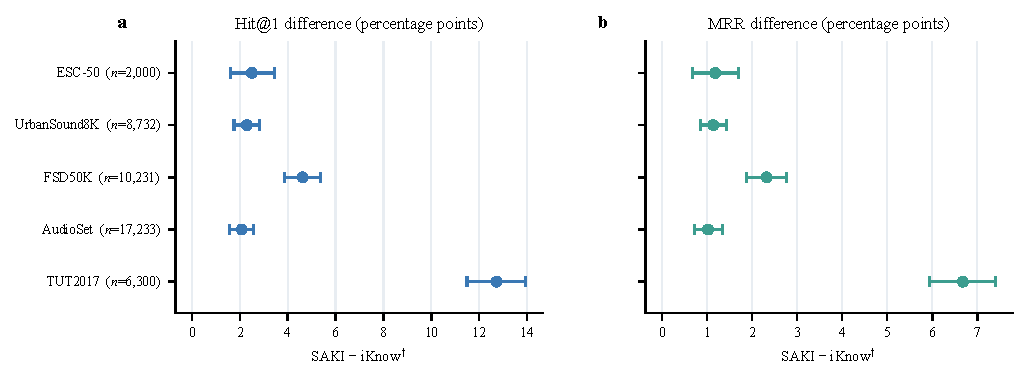
\includegraphics[width=0.80\textwidth]{figures/further_analysis/fig_statistical_significance.pdf}
    \caption{Paired Hit@1 and MRR differences between SAKI and iKnow\textsuperscript{\dag}, with 95\% confidence intervals. Points denote observed differences; error bars are obtained from 10,000 paired bootstrap resamples of test audio. The vertical dashed line marks zero difference. The horizontal axis is in percentage points.}
    \label{fig:statistical-significance}
\end{figure}
\end{minipage}
\end{figure*}

\subsubsection{Knowledge verbalization analysis}\label{sec:verbalization-analysis}


We compare three knowledge text representations under the same relation selection algorithm and Hierarchical Fusion rules. Direct concatenation joins class names and tail entities; Raw triple retains the class, relation, and tail fields. AAKV organizes triples into sound descriptions that preserve entity and relation semantics. Each configuration computes relation-specific class scores from its own texts, allowing representation choices to be compared within the same inference procedure.

Table~\ref{tab:knowledge-verbalization} shows that AAKV achieved higher Hit@1 than both controls on all five datasets. Its unweighted mean Hit@1 and MRR reached 66.81\% and 75.08\%, exceeding Direct concatenation by 3.18 and 1.77 percentage points. Raw triple yielded mean Hit@1 and MRR of 63.46\% and 72.91\%, slightly below Direct concatenation's 63.63\% and 73.31\%. Simply adding relation fields thus provided limited benefit in this experiment, suggesting that their textual organization also matters.

ReCLAP expands class semantics through acoustic descriptions and prompts covering diverse scenes, and reports improved zero-shot classification with prompt augmentation~\cite{ghosh2024reclap}. Our verbalization comparison likewise supports the importance of text representation, although AAKV specifically expresses existing triple relations as constrained sound descriptions. Natural-language sentences explicitly connect the class, relation, and tail entity, providing CLAP's text encoder with a coherent semantic expression. This may help explain AAKV's gains over \greenrevision{text consisting of separate triple fields}.

\bluerevision{Relative to Direct concatenation, AAKV increased Hit@1 by 3.86 percentage points on FSD50K and 9.00 on TUT2017, compared with 0.35 on ESC-50. On ESC-50, its MRR was comparable to Raw triple (95.75\% versus 95.77\%).}



\subsection{Further analysis}\label{sec:further-analysis}

We examine uncertainty in performance differences, sample-level prediction transitions, parameter selection, and computational cost.



\subsubsection{Statistical significance}\label{sec:statistics}

\redrevision{We assess uncertainty in the Hit@1 and MRR gains of SAKI over iKnow\textsuperscript{\dag} using paired bootstrap confidence intervals.} Following the paired bootstrap procedure in Section~\ref{sec:evaluation-metrics}, we use the same resampled audio indices for both methods. The 2.5th and 97.5th percentiles of the difference distribution define the 95\% confidence interval.

In Figure~\ref{fig:statistical-significance}, all observed Hit@1 and MRR differences are positive, and their 95\% confidence intervals lie entirely above zero. TUT2017 shows the largest Hit@1 gain, at 12.73 percentage points, with a confidence interval of [11.49, 13.95] percentage points. The intervals on the other datasets also exclude zero, supporting the observed gains under resampling of the current test audio.

\bluerevision{These intervals reflect uncertainty from resampling test samples, with the models and inference settings held fixed.}


\subsubsection{\nextrevision{Prediction transitions and case study}}\label{sec:cases}

\redrevision{Transitions from incorrect iKnow\textsuperscript{\dag} predictions to correct SAKI predictions outnumbered the reverse transitions on all five datasets. The difference yielded a net improvement in top-1 accuracy.} On FSD50K, for example, 991 incorrect predictions became correct, while 518 correct predictions became incorrect. Reranking therefore corrected errors while also changing some originally correct decisions. The gains in the main table summarize the net effect of both changes.

\begin{figure}[H]
    \centering
    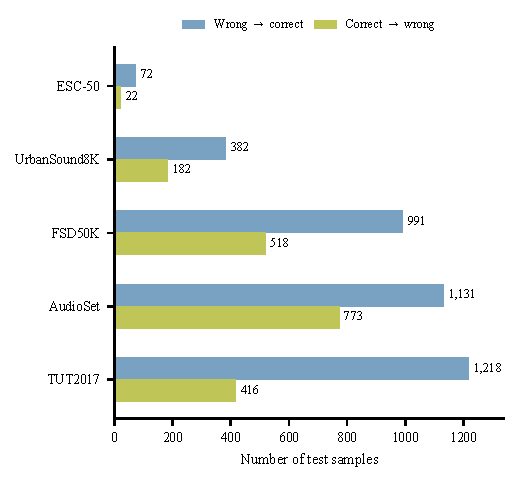
\includegraphics[width=0.84\columnwidth]{figures/further_analysis/fig_prediction_transitions.pdf}
    \caption{Sample-level Hit@1 transitions from iKnow\textsuperscript{\dag} to SAKI. Blue bars count \greenrevision{transitions from incorrect to correct predictions}; yellow-green bars count \greenrevision{transitions from correct to incorrect predictions}. Their difference is the net increase in correct predictions with SAKI.}
    \label{fig:prediction-transitions}
\end{figure}

Figure~\ref{fig:prediction-transitions} decomposes the overall Hit@1 gains into error corrections and prediction degradations.

We applied two-sided exact McNemar tests to the discordant pairs shown in the figure. All five $p$ values remained below 0.05 after Holm adjustment, with a maximum of approximately $2.26\times10^{-7}$ (Table~\ref{tab:mcnemar-tests}). Together with the transition directions, these results support SAKI's Hit@1 advantage after controlling the familywise error rate across the five tests.

Table~\ref{tab:case-study} illustrates three types of ranking changes. In the correction case, \textit{wind} moved from fifth to first. In the \greenrevision{case of improved ranking}, \textit{sea waves} rose from third to second, while SAKI predicted \textit{frog} at rank one. In the degradation case, \textit{washing machine} fell from first to fourth, and SAKI instead predicted \textit{engine}.

\begin{table}[H]

\centering

\caption{Three representative prediction changes on ESC-50. Parentheses give the ground-truth class rank. \redrevision{The cached evidence texts are reproduced verbatim and provide examples of evidence read for candidate classes during inference.} They do not establish the independent contribution of an individual evidence item to the prediction change.}

\label{tab:case-study}

\footnotesize

\setlength{\tabcolsep}{2pt}

\begin{tabular*}{\columnwidth}{@{\extracolsep{\fill}}llll@{}}

\toprule

Case & True class & iKnow\textsuperscript{\dag} & SAKI \\

\midrule

Correction
& wind & train (5) & wind (1) \\

\multicolumn{4}{@{}p{\columnwidth}@{}}
{\textit{AAKV evidence: The sound of wind is instance of ocean.}} \\

\addlinespace[2pt]

Rank improvement
& sea waves & crickets (3) & frog (2) \\

\multicolumn{4}{@{}p{\columnwidth}@{}}
{\textit{AAKV evidence: The sound of frog is part of a wetland scene.}} \\

\addlinespace[2pt]

Degradation
& washing machine & washing machine (1) & engine (4) \\

\multicolumn{4}{@{}p{\columnwidth}@{}}
{\textit{AAKV evidence: The sound of engine is instance of motorcycle.}} \\

\bottomrule

\end{tabular*}

\end{table}

These cases illustrate how Hit@1 and MRR capture different ranking changes. Moving \textit{wind} to first improves both metrics. For \textit{sea waves}, reciprocal rank increases from $1/3$ to $1/2$, while Hit@1 remains zero. Moving \textit{washing machine} away from first reduces both metrics. Reporting Hit@1 and MRR together thus distinguishes error correction, rank improvement below first place, and prediction degradation.

Prediction degradation also highlights the limits of relation consensus. \redrevision{Class scores for all relations are computed using the same CLAP encoder. Agreement among their top-1 predictions may therefore reflect matching biases shared by the underlying model.} Consensus and larger top-two score gaps provide selection criteria, but do not establish evidence correctness or relevance to the sample.

\Needspace{8\baselineskip}
\subsubsection{Parameter sensitivity}\label{sec:parameters}

We examine the fusion weight $\alpha$ and relation count $N_r$ on the DCASE17-T4 development set. The search range and selection rule are given in Section~\ref{sec:implementation-details}.

\begin{figure}[H]
    \centering
    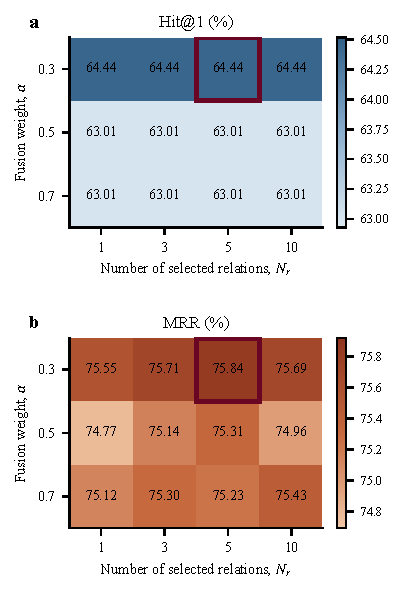
\includegraphics[width=0.80\columnwidth]{figures/further_analysis/fig_parameter_sensitivity.pdf}
    \caption{Parameter sensitivity on the DCASE17-T4 development set. (a) Hit@1 for different fusion weights $\alpha$ and relation counts $N_r$. (b) MRR for the same configurations. The outlined configuration, $\alpha=0.3$ and $N_r=5$, is selected by maximizing Hit@1 and then MRR.}
    \label{fig:parameter-sensitivity}
\end{figure}

Figure~\ref{fig:parameter-sensitivity}(a) shows identical Hit@1 for all four relation counts at each fixed $\alpha$. Hit@1 was 64.44\% at $\alpha=0.3$, compared with 63.01\% at $\alpha=0.5$ or $0.7$. Within this search range, top-1 accuracy varied with the fusion weight but remained unchanged across relation counts.

MRR distinguishes configurations with identical Hit@1 (Figure~\ref{fig:parameter-sensitivity}(b)). At $\alpha=0.3$, increasing $N_r$ from one to five raised MRR from 75.55\% to 75.84\%; increasing it to ten reduced MRR to 75.69\%. \redrevision{The benefit of adding relations was therefore nonmonotonic within the tested range.} Following the \greenrevision{predefined rule for choosing parameters on the development set}, we selected $\alpha=0.3$ and $N_r=5$ and fixed them for all five test datasets.


\Needspace{30\baselineskip}
\subsubsection{Computational cost analysis}\label{sec:computational-cost}
\begin{table}[!t]
\centering
\caption{Online inference efficiency and offline cache size at batch size 1. Latency, peak GPU memory, and cache size are unweighted means across the five test datasets. Relative overhead is the ratio to mean CLAP latency; throughput is computed from mean latency.}
\label{tab:computational-cost}
\small
\setlength{\tabcolsep}{4pt}
\begin{tabular}{lccc}
\toprule
Metric & CLAP & iKnow\textsuperscript{\dag} & SAKI \\
\midrule
Latency (ms/sample) & 24.37 & 25.16 & 86.52 \\
Relative overhead & 1.00$\times$ & 1.03$\times$ & 3.55$\times$ \\
Throughput (samples/s) & 41.03 & 39.74 & 11.56 \\
Peak GPU memory usage (MiB) & 693.60 & 700.30 & 743.22 \\
Offline cache (MiB) & 0.63 & 6.74 & 50.52 \\
\bottomrule
\end{tabular}
\end{table}

We compare the three methods on identical hardware and test samples. \redrevision{For each dataset, we selected 200 fixed samples and processed 20 samples for warm-up. We then repeated timing five times at batch size one.} Online time includes audio preprocessing, CLAP audio encoding, scoring, and ranking. RotatE retrieval, AAKV generation, and text encoding are performed offline. Table~\ref{tab:computational-cost} reports unweighted mean latency, peak GPU memory usage, and cache size across the five datasets. Relative overhead and throughput are calculated from mean latency. The cache includes text embeddings and evidence index mappings, excluding model weights, raw audio, and the source knowledge graph.



Table~\ref{tab:computational-cost} shows that iKnow\textsuperscript{\dag}'s latency of 25.16~ms/sample was close to CLAP's 24.37~ms/sample. SAKI required 86.52~ms/sample, corresponding to 3.55 times CLAP's latency and a throughput of 11.56 samples/s. Peak GPU memory usage was 743.22~MiB for SAKI and 693.60~MiB for CLAP; offline caches were 50.52 and 0.63~MiB, respectively. \redrevision{Relative to CLAP, SAKI showed a smaller proportional increase in peak GPU memory usage than in latency, while its cache size increased substantially.} In these measurements, deployment costs mainly involved longer online processing and greater storage for precomputed evidence. \greenrevision{SAKI also performs relation-specific scoring, relation ranking, and evidence fusion online, consistent with its higher measured latency.}

\subsection{Limitations}\label{sec:limitations}

SAKI's applicability depends on both knowledge quality and the underlying model. AAKV constrains how triples are expressed, while retrieval errors and associations irrelevant to the current audio can still enter the classification evidence. The current evaluation uses fixed MS-CLAP 2023 and RotatE models and 47 candidate relations. The observed gains apply to these resources and the five test datasets; transfer to other audio--language models and knowledge graphs requires further evaluation.

Online relation evaluation also increases inference time and cache requirements, limiting the flexibility of the current implementation in low-latency settings. Future work can assess evidence reliability to reduce unsuitable knowledge and use lightweight relation preselection to reduce the number of evaluated relations. These directions seek a more favorable balance between classification performance and inference cost.


\FloatBarrier

% !TeX root = ../main-4.tex
\section{Conclusion}\label{sec:conclusion}

\teacherrevision{This work shows that adapting graph knowledge to individual clips can improve zero-shot audio classification.} We proposed SAKI, which combines sample-level relation selection, constrained knowledge verbalization, and Hierarchical Fusion to rerank candidate classes without updating CLAP parameters. \teacherrevision{SAKI improved Hit@1 and MRR over iKnow\textsuperscript{\dag} on all five public test datasets.} It also achieved the highest unweighted mean Hit@1 and MRR in the component ablations. \redrevision{Under the evaluated settings, these findings support coordinating sample relevance, text representation, and score fusion when incorporating structured knowledge into pretrained audio--language models.} Future work will examine evidence reliability and lightweight relation selection, and assess applicability across different audio--language models and knowledge graphs.


\section*{Acknowledgments}
This work was supported in part by the Wenzhou Basic Scientific Research Projects under Grant 2025G0082.

\section*{Declaration of competing interest}
The authors declare that they have no known competing financial interests or personal relationships that could have appeared to influence the work reported in this paper.

\section*{Data availability}
The datasets used in this study are publicly available, including ESC-50, UrbanSound8K, DCASE17-T4, FSD50K, AudioSet, and TUT2017. The processed data and implementation details will be made available by the corresponding authors upon reasonable request.

\begingroup
\small
\setlength{\bibsep}{0pt}
\bibliographystyle{elsarticle-num}
\bibliography{references_main4}
\endgroup

% KBS/Elsevier appendices follow the reference list.
\appendix
% !TeX root = ../main-4.tex
\onecolumn
\raggedbottom
\small
\renewcommand{\theHtable}{appendix.\thesection.\arabic{table}}
\setlength{\parskip}{0pt}
\setlength{\intextsep}{5pt plus 1pt minus 1pt}
\setlength{\textfloatsep}{6pt plus 1pt minus 1pt}
\begin{multicols}{2}
\raggedcolumns
\section{\methodrevision{AAKV generation and validation protocol}}\label{app:aakv-protocol}
\methodrevision{For each retrieved triple, the generator receives a system instruction and a user message containing the three fields \texttt{[head]}, \texttt{[relation]}, and \texttt{[tail]}. \greenrevision{The \texttt{[head]} field contains the candidate class name $c_i$, corresponding to the graph entity $h_i$ used for retrieval. The placeholder \texttt{\{head\}} is replaced with this class name.} The full system instruction used in the implementation is reproduced below.}

\begin{quote}
\methodrevision{You are a faithful knowledge-graph verbalizer for an audio-text matching model. Convert exactly one knowledge-graph triple into one short, natural English sentence about sound.}

\methodrevision{Rules:}
\begin{enumerate}
\item \methodrevision{Begin the sentence with exactly: ``The sound of \texttt{\{head\}}''. Replace \texttt{\{head\}} with the supplied head text exactly.}
\item \methodrevision{Use only information explicitly contained in the triple.}
\item \methodrevision{Preserve the head entity, relation meaning, relation direction, and tail entity.}
\item \methodrevision{Preserve the original wording of the head and tail. Do not pluralize, abbreviate, replace, or omit either entity.}
\item \methodrevision{Do not add acoustic properties, causes, locations, purposes, examples, explanations, or external knowledge.}
\item \methodrevision{Do not correct or reinterpret the factual content, even if it seems unusual.}
\item \methodrevision{Add only grammatical function words such as articles, prepositions, and forms of ``be''.}
\item \methodrevision{Silently verify that the sentence expresses exactly the supplied triple.}
\item \methodrevision{Output only one final sentence, without reasoning, labels, headers, or quotation marks.}
\end{enumerate}
\end{quote}

\methodrevision{The user message has the exact field layout \texttt{[head] head}, \texttt{[relation] relation}, and \texttt{[tail] tail}, with each field on a separate line. Qwen2.5-7B-Instruct is decoded greedily (\texttt{do\_sample=False}, \texttt{max\_new\_tokens=48}). The rule-based check tests the required prefix, lexical coverage of the head and tail, \greenrevision{coverage of terms denoting the relation}, a maximum of 30 words, a single line and sentence, and the absence of \greenrevision{prohibited formatting and acoustic property terms}. These checks assess observable text constraints; they do not constitute a semantic proof of triple fidelity.}

\methodrevision{If the first output fails, the model receives its preceding output, \greenrevision{the reasons for failure}, and the following repair instruction: ``Your preceding sentence failed an automatic fidelity check. Rewrite it as exactly one short English sentence beginning with the exact words `The sound of \texttt{\{head\}}'. Copy the supplied head and tail text exactly and explicitly express the supplied relation in its original direction. Do not add, correct, explain, or infer anything. Output only the sentence.'' If the repaired output still fails, the implementation uses the deterministic fallback ``The sound of \texttt{\{head\}} has the relation \texttt{\{relation\}} with \texttt{\{tail\}}.''}

\end{multicols}
\section{Controlled reimplementation and dataset protocols}\label{app:reproduction}

\setcounter{table}{0}
\renewcommand{\thetable}{B.\arabic{table}}

\subsection{Dataset protocol reconciliation}

\begin{table}[H]
\centering
\caption{\purplerevision{Dataset protocols reported by iKnow-audio and used in this work. The sample counts document protocol differences; absolute performance across the two protocols is not treated as directly comparable.}}
\label{tab:dataset-reconciliation}
\fontsize{9}{11}\selectfont
\setlength{\tabcolsep}{4pt}
\begin{tabular}{lrrlp{0.55\textwidth}}
\toprule
Dataset & iKnow-audio & This work & Role & Protocol note \\
\midrule
ESC-50 & 2,000 & 2,000 & Test & The full dataset is used. All 2,000 files in our evaluation manifest \greenrevision{pass the audio decoding check}. \\
UrbanSound8K & 8,732 & 8,732 & Test & The full dataset is used. All 8,732 files in our evaluation manifest \greenrevision{pass the audio decoding check}. \\
FSD50K & 20,462 & 10,231 & Test & We use the official FSD50K evaluation split containing 10,231 clips. The iKnow-audio paper reports 20,462 test items; therefore absolute results across the two protocols are not treated as directly comparable. \\
AudioSet & 20,371 & 17,233 & Test & Our fixed evaluation manifest contains 17,233 available and readable audio files. The exact manifest will be released for reproducibility. \\
TUT2017 & 6,300 & 6,300 & Test & We use all 6,300 clips from the development (4,680) and evaluation (1,620) partitions. \\
DCASE17-T4 & 488 & 419 & Development & Our fixed development manifest contains 419 readable clips and is used only for selecting $\alpha$ and $N_r$. It is excluded from the five final test datasets. \\
\bottomrule
\end{tabular}
\end{table}

\Needspace{26\baselineskip}
\subsection{iKnow\textsuperscript{\dag} controlled reimplementation protocol}

\begin{table}[H]
\centering
\caption{\purplerevision{Correspondence between the original iKnow-audio method and the iKnow\textsuperscript{\dag} controlled reimplementation protocol in this work.}}
\label{tab:iknow-protocol}
\fontsize{9}{11}\selectfont
\setlength{\tabcolsep}{4pt}
\begin{tabular}{>{\raggedright\arraybackslash}p{0.16\textwidth}>{\raggedright\arraybackslash}p{0.27\textwidth}>{\raggedright\arraybackslash}p{0.23\textwidth}>{\raggedright\arraybackslash}p{0.27\textwidth}}
\toprule
Component & Original iKnow-audio & iKnow\textsuperscript{\dag} in this work & Treatment \\
\midrule
Relation set & \nextrevision{Curated informative relations $R_q \subset R$} & \greenrevision{Fixed relations reconstructed for each dataset} & \purplerevision{The complete original $R_q$ is not publicly available} \\
Knowledge graph & Audio-centric Knowledge Graph (AKG) & AKG resource used in our reimplementation & Kept fixed across internal comparisons \\
KGE model & \purplerevision{RotatE for tail prediction} & \purplerevision{Pretrained RotatE for tail prediction} & \purplerevision{Same model family; fixed across internal comparisons} \\
Candidate classes & CLAP top-ranked candidate classes & Top-$K$, $K=5$ & Unified across iKnow\textsuperscript{\dag} and ablation branches \\
Tail retrieval & Top-ranked tail entities & Top-$M$, $M=3$ & Unified across iKnow\textsuperscript{\dag} and ablation branches \\
Knowledge text & \purplerevision{Class--tail concatenation} & Direct class--tail concatenation & \purplerevision{Same construction in principle; baseline text representation} \\
Score aggregation & \redrevision{Log-sum-exp over original CLAP and knowledge-augmented prompt scores} & Normalized scaled log-sum-exp, $\methodrevision{\lambda}=100$ & \purplerevision{Controlled modification shared by iKnow\textsuperscript{\dag} and ablations} \\
Evaluation samples & Original paper protocol & Fixed manifests in Table~\ref{tab:dataset-reconciliation} & All methods in this work use identical manifests and evaluation code \\
\bottomrule
\end{tabular}
\end{table}

\Needspace{20\baselineskip}
\section{Additional ablation results}\label{app:ablation}
\setcounter{table}{0}
\renewcommand{\thetable}{C.\arabic{table}}

Table~\ref{tab:ablation-topk} supplements the component ablations with Hit@3 and Hit@5. The configurations and all other settings match Table~\ref{tab:factorial-ablation}.

\begin{table}[H]
\centering
\caption{Hit@3 and Hit@5 (\%) for the eight configurations in Table~\ref{tab:factorial-ablation}. Higher is better. \greenrevision{The mean across the five datasets is unweighted.} Fusion and Selector abbreviate Hierarchical Fusion and Sample-level Relation Selector.}
\label{tab:ablation-topk}
\setlength{\tabcolsep}{2.5pt}
\resizebox{\textwidth}{!}{%
\begin{tabular}{l*{12}{c}}
\toprule
\multirow{2}{*}{Method}
& \multicolumn{2}{c}{ESC-50}
& \multicolumn{2}{c}{UrbanSound8K}
& \multicolumn{2}{c}{FSD50K}
& \multicolumn{2}{c}{AudioSet}
& \multicolumn{2}{c}{TUT2017}
& \multicolumn{2}{c}{\greenrevision{Mean (5 datasets)}} \\
\cmidrule(lr){2-3}\cmidrule(lr){4-5}\cmidrule(lr){6-7}\cmidrule(lr){8-9}\cmidrule(lr){10-11}\cmidrule(lr){12-13}
& Hit@3 & Hit@5 & Hit@3 & Hit@5 & Hit@3 & Hit@5 & Hit@3 & Hit@5 & Hit@3 & Hit@5 & Hit@3 & Hit@5 \\
\midrule
iKnow\textsuperscript{\dag}
& 97.05 & 97.65 & 96.77 & 98.65 & 80.73 & 86.51 & 47.04 & 54.87 & 79.89 & 92.68 & 80.30 & 86.07 \\
+ AAKV
& 95.90 & 97.65 & 96.14 & 98.65 & 80.63 & 86.46 & 46.73 & 54.80 & 79.65 & 92.27 & 79.81 & 85.97 \\
+ Fusion
& 97.10 & 97.65 & 96.86 & 98.65 & 81.24 & 86.67 & 47.48 & 55.14 & 80.78 & 92.65 & 80.69 & 86.15 \\
+ Selector
& 97.05 & 97.70 & 96.36 & 98.65 & 79.96 & 86.38 & 46.68 & 55.00 & 80.83 & 92.52 & 80.17 & 86.05 \\
+ AAKV + Fusion
& 97.00 & 97.65 & 96.56 & 98.65 & 81.21 & 86.58 & 47.10 & 54.93 & 81.30 & 92.00 & 80.64 & 85.96 \\
+ AAKV + Selector
& 96.30 & 97.65 & 96.09 & 98.65 & \methodrevision{80.09} & \methodrevision{86.40} & \methodrevision{46.61} & 54.90 & 79.56 & 92.25 & \methodrevision{79.73} & 85.97 \\
+ Fusion + Selector
& 97.05 & 97.65 & 96.60 & 98.65 & 79.68 & 86.38 & 46.34 & 54.94 & 80.70 & 92.63 & 80.07 & 86.05 \\
SAKI
& 96.80 & 97.65 & 96.90 & 98.65 & \methodrevision{80.52} & \methodrevision{86.48} & \methodrevision{46.90} & \methodrevision{54.80} & 80.54 & 91.79 & \methodrevision{80.33} & 85.88 \\
\bottomrule
\end{tabular}
}
\end{table}

\begin{table}[H]
\centering
\caption{Relations selected by Frequency Top-5 for each dataset. Relations are ranked by the number of class--tail evidence entries in the offline cache.}
\label{tab:frequency-relations}
\setlength{\tabcolsep}{4pt}
\begin{tabular}{lp{0.82\textwidth}}
\toprule
Dataset & Frequency Top-5 relations \\
\midrule
ESC-50 & \texttt{can be heard in}; \texttt{has duration}; \texttt{localized in}; \texttt{part of scene}; \texttt{associated with environment} \\
UrbanSound8K & \texttt{affects}; \texttt{associated with environment}; \texttt{associated with event}; \texttt{can be heard in}; \texttt{co-occurs with} \\
FSD50K & \texttt{associated with environment}; \texttt{can be heard in}; \texttt{localized in}; \texttt{occurs in}; \texttt{part of scene} \\
AudioSet & \texttt{can be heard in}; \texttt{occurs in}; \texttt{localized in}; \texttt{described by}; \texttt{associated with environment} \\
TUT2017 & \texttt{affects}; \texttt{associated with environment}; \texttt{can be heard in}; \texttt{co-occurs with}; \texttt{emotionally associated with} \\
\bottomrule
\end{tabular}
\end{table}


\section{Sample-level relation selection behavior}\label{app:selector-behavior}
\setcounter{table}{0}
\renewcommand{\thetable}{D.\arabic{table}}

\begin{table}[H]
\centering
\caption{\purplerevision{Sample-level relation selection behavior on the five test datasets. Combinations containing the same five relations are counted as one set, regardless of their order. Dominant-set share is the percentage of samples using the most frequent set.} \greenrevision{Mean Jaccard measures set overlap with the complete FrozenRq relation set for each dataset, not classification performance.}}
\label{tab:selector-behavior}
\small
\setlength{\tabcolsep}{6pt}
\begin{tabular}{lrrrr}
\toprule
Dataset & \#Samples & \#Unique Top-5 sets & Dominant-set share (\%) & \redrevision{\shortstack{Mean Jaccard similarity\\with FrozenRq}} \\
\midrule
ESC-50 & 2,000 & 1,708 & 1.40 & 0.0405 \\
UrbanSound8K & 8,732 & 5,461 & 1.53 & 0.0739 \\
FSD50K & 10,231 & \methodrevision{9,069} & \methodrevision{1.52} & \methodrevision{0.0559} \\
AudioSet & 17,233 & \methodrevision{15,733} & \methodrevision{1.38} & \methodrevision{0.0581} \\
TUT2017 & 6,300 & 4,336 & 1.06 & 0.0636 \\
\bottomrule
\end{tabular}
\end{table}

\section{\nextrevision{Paired Hit@1 test results}}\label{app:mcnemar-tests}
\setcounter{table}{0}
\renewcommand{\thetable}{E.\arabic{table}}

\nextrevision{Table~\ref{tab:mcnemar-tests} reports the exact two-sided McNemar tests for SAKI versus iKnow\textsuperscript{\dag} on the final evaluation samples. The test uses only discordant Hit@1 outcomes; Holm adjustment is applied across the five datasets.}

\begin{table}[H]
\centering
\color{black}
\caption{\purplerevision{Paired Hit@1 transitions and significance tests for SAKI versus iKnow\textsuperscript{\dag}. \redrevision{Incorrect $\to$ correct denotes an incorrect iKnow\textsuperscript{\dag} prediction and a correct SAKI prediction; correct $\to$ incorrect denotes the reverse.} Two-sided exact McNemar $p$ values are adjusted across five datasets using the Holm method.}}
\label{tab:mcnemar-tests}
\fontsize{9}{11}\selectfont
\setlength{\tabcolsep}{4pt}
\begin{tabular}{lrrrrr}
\toprule
Dataset & $n$ & \redrevision{\shortstack{Incorrect\\$\to$ correct}} & \redrevision{\shortstack{Correct\\$\to$ incorrect}} & $p_{\mathrm{exact}}$ & $p_{\mathrm{Holm}}$ \\
\midrule
ESC-50 & 2,000 & 72 & 22 & $2.26\times10^{-7}$ & $2.26\times10^{-7}$ \\
UrbanSound8K & 8,732 & 382 & 182 & $2.47\times10^{-17}$ & $7.41\times10^{-17}$ \\
FSD50K & 10,231 & 991 & 518 & $1.63\times10^{-34}$ & $6.51\times10^{-34}$ \\
AudioSet & 17,233 & 1,131 & 773 & $2.30\times10^{-16}$ & $4.59\times10^{-16}$ \\
TUT2017 & 6,300 & 1,218 & 416 & $3.52\times10^{-91}$ & $1.76\times10^{-90}$ \\
\bottomrule
\end{tabular}
\end{table}


\end{document}
